\documentclass{report}

\usepackage[portuguese]{babel}

\usepackage[letterpaper,top=2cm,bottom=2cm,left=3cm,right=3cm,marginparwidth=1.75cm]{geometry}

% Useful packages
\usepackage{amsmath}
\usepackage{graphicx}
\graphicspath{ {./images/} }
\usepackage[colorlinks=true, allcolors=blue]{hyperref}
\usepackage{etoolbox}
\patchcmd{\abstract}{\null\vfil}{}{}{}

\usepackage{lipsum}


\title{Google TPU}
\author{Fernando Lima \\ Isabella Caselli \\ Rodrigo Michelassi}
\date{2024}

\begin{document}
\maketitle
\tableofcontents	% como colocar isso na mesma pagina que o titulo

% --- ABSTRACT --- % 
\begin{abstract}
Na era do desenvolvimento de sistemas baseados em Inteligência Artificial e redes neurais profundas (Deep Learning), se faz necessário o uso de máquinas super potentes, capazes de processar dados e realizar operações matemáticas de maneira extremamente rápida. Modelos de Machine Learning podem levar horas, até mesmo dias, para serem treinados, devido principalmente a operações como produto interno entre matrizes e a enorme quantidade de dados que são usados, trazendo um prejuízo não apenas de tempo, mas também energético, ambiental e sobretudo lucrativo. Nesse artigo, iremos tratar brevemente sobre a utilização de Cloud TPUs, unidades de processamento de tensores do Google Cloud, que atuam na otimização do treinamento de modelos de aprendizado de máquina, e que se tornou indispensável na academia e na indústria, para todos estudiosos e profissionais da área.
\end{abstract}

% --- CHAPTER 1 --- % 
\chapter{Introdução}

A evolução da tecnologia tem proporcionado diversos avanços no campo da inteligência artificial, principalmente no desenvolvimento de redes neurais profundas (Deep Learning) e aprendizado de máquina. Nesse cenário, a demanda por maior poder computacional levou à criação de hardware especializado, capaz de lidar com a complexidade e o volume de cálculos necessários para essas tarefas. Nesse contexto, destaca-se a Unidade de Processamento Tensorial (TPU), um circuito integrado de aplicação específica (ASIC) desenvolvido pelo Google.

As TPUs, lançadas em 2015, foram projetadas para acelerar operações de aprendizado de máquina, otimizando o treinamento de modelos baseados em redes neurais. Diferentemente de CPUs e GPUs, cuja arquitetura é projetada para fins generalistas, as TPUs são especializadas em multiplicações e somas de matrizes, que são operações fundamentais em áreas como Deep Learning. Essa especialização confere às TPUs maior eficiência energética e desempenho significativamente superior em tarefas relacionadas à inteligência artificial.

Dessa forma, considerando o tema apresentado como essencial para os avanços significativos que foram alcançados nas áreas de IA e Aprendizado de Máquina, este trabalho se propõe a explorar a arquitetura, os princípios de funcionamento e as aplicações das TPUs no contexto da computação moderna. 

% --- CHAPTER 2 --- % 
\chapter{História}

A Google Tensor Processing Unit é uma arquitetura de circuito integrado conhecido como um "acelerador de IA". Essa arquitetura tem seu início em $2016$, como uma alternativa a outras estruturas já conhecidas, utilizadas popularmente para acelerar o treinamento de modelos de IA, como as GPUs e os arrays sistólicos.

Apesar dessa tecnologia ser divulgada ao público apenas em $2016$, engenheiros da Google divulgaram que já era utilizada há mais de um ano em datacenters da big tech. Essa arquitetura foi pensada para funcionar juntamente a biblioteca de Machine Learning da Google, o TensorFlow, utilizada para treinar grandes modelos baseados em redes neurais, e atualmente uma das maiores bibliotecas do ramo. 

Entre as principais atividades executadas pela TPU está o processamento de tensores, estrutura de dados conhecida como um array multidimensional. Dessa forma, estratégias diversas para multiplicação de tensores (linear e paralelamente) são comumente estudadas em diversos campos da matemática clássica, dentro da Álgebra Linear, e as mais modernas arquiteturas para processamentos de produtos matriciais se baseiam em técnicas já conhecidas.

Atualmente, as TPUs são proprietárias, e no geral o acesso se limita a própria Google ou usuários que pagam por seu uso. É possível que empresas contratem o serviço por meio do sistema de nuvem da Google ou utilizem através do Google Colab, com tempo limitado de uso ou aluguel de TPUs mais potentes.

% --- CHAPTER 3 --- % 
\section{Tensores}

% --- CHAPTER 4 --- % 
\section{Aprendizado de Máquina e Redes Neurais}

Nos tempos de ChatGPT, IA's generativas, problemas éticos com uso de imagens e dados pessoais por grandes empresas, surge a necessidade de se entender como funcionam os modelos de Aprendizado de Máquina. 

Nesse sentido, o surgimento das TPUs estão associadas justamente oa fortalecimento científico e comercial desse tipo de tecnologia, que a cada dia vem sendo explorada mais fortemente, e utilizando grandes camadas de dados. Esses modelos exigem muito poder computacional para processar todos os dados fornecidos, além de realizar diversas operações matemáticas como produtos tensoriais. 

De maneira resumida, modelos de Aprendizado de Máquina no geral consiste na modelagem matemática de problemas, com propósitos variáveis, mas que todos possuem algo em comum: fazer com que o modelo se ajuste bem, a ponto de dar respostas boas para suas entradas. Dessa forma, se percebe uma boa semelhança com a computação clássica, dada uma entrada, processamos uma respectiva saída. Todavia, esses modelos são probabilísticos, e não há garantia que a resposta sempre será a esperada. Para que servem esses modelos, então?

Há problemas que são fáceis para humanos responderem, mas difíceis de serem automatizados. Por exemplo, dada uma imagem de um gato, um ser humano pode facilmente ver a imagem e dizer "essa é uma imagem de um gato". Porém, se existisse a necessidade de automatizar tal tarefa? Como podemos escrever um algoritmo que, dada uma imagem, de qualquer tamanho e padrão de cores, apenas utilizando ferramentas clássicas de algoritmos (loops, condicionais) e dizer se aquela imagem contém de fato, um gato? Nesse contexto, utilizar Machine Learning é uma boa ideia.

Adicionalmente, os modelos mais modernos de Aprendizado de Máquina estão atrelados ao desenvolvimento de redes neurais. Esses modelos são treinados baseados em dois passos, conhecidos como forward e back-propagation. Redes Neurais são constituídas por nós, representando features de dados, e pesos atribuídos a cada uma dessas features, e a operação de Forward-Propagation consiste em realizar produtos vetoriais entre esses pesos com o valor dos nós (função não linear da soma ponderada dos dados de entrada). A operação de Back-Propagation deve retornar a rede neural, atualizando os pesos com base no erro calculado, novamente utilizando operações de produtos vetoriais. Note que essas operações são extremamente custosas, e Redes Neurais possuem milhares, até milhões de parâmetros, a depender do modelo, e é necessário acelerar esse processamento, com base em paralelismo e busca de algoritmos mais eficientes.

\begin{figure}[h]
	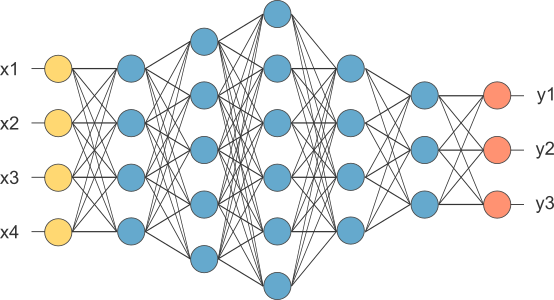
\includegraphics[scale=0.7]{neuralNetwork}
	\centering
	\caption{Estrutura gráfica de uma Rede Neural}
\end{figure}

Com base nisso, temos um modelo matemático, que atualiza pesos e é capaz de responder perguntas, porém se ele nem sempre acerta, como eles são de fato utilizados? Vimos que modelos de Aprendizado de Máquina são baseados matemáticos e baseados em pesos. Existem diversas aplicações para esses modelos, e o trabalho de um engenheiro de Machine Learning é conseguir treinar um modelo, com dados o suficiente, de forma a minimizar o erro desse modelo, dessa forma aumentando sua acurácia e garantindo que o modelo tenha uma maior probabilidade de acertar as respostas, com base nos dados que são utilizados como entrada. Atualmente, esses modelos tem diversos usos na indústria, como no mercado financeiro, para predição de séries temporais para variações da bolsa de valores, na medicina para auxílio de profissionais no diagnóstico de doenças, no direito para análise textual de casos, na astronomia, como na recente descoberta da primeira imagem de um buraco negro. 

Dessa forma, Machine Learning é uma tendência que cresce tanto no mercado como na academia, e deve continuar sendo explorado por diversos profissionais, de forma que é necessário acelerar o longo processo de treinamento de modelos, além de buscar soluções mais sustentáveis para que o conhecimento possa continuar se expandindo.


% --- CHAPTER 5 --- % 
\chapter{Arquitetura da TPU}

As TPUs surgem como uma alternativa de arquitetura simples para o usuário, de forma que tenha uma interface de hardware mais amigável, ao mesmo tempo que consegue processar dados mais rapidamente, atingindo as demandas necessárias em $2015$ para processamento de redes neurais. Essa arquitetura foi desenhada para processar dados de maneira independente da CPU, e recebe instruções de processamento do servidor onde está conectado.

\begin{figure}[h]
	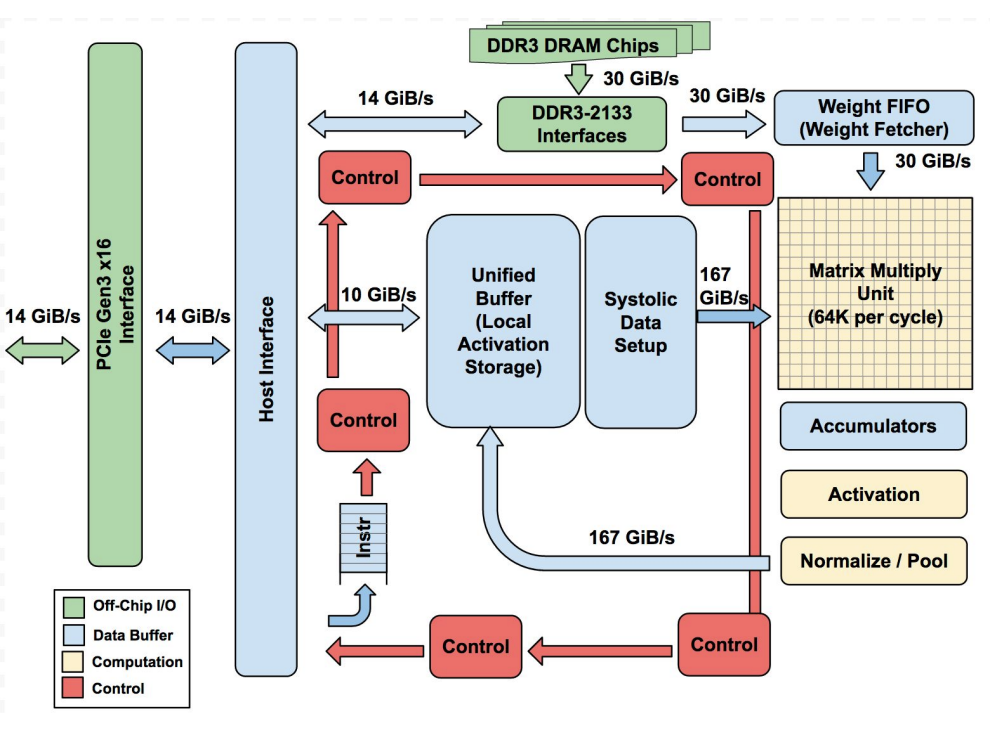
\includegraphics[scale=0.7]{tpu-block-diagram}
	\centering
	\caption{Estrutura básica de uma TPU}
\end{figure}

Para entender melhor a arquitetura de uma TPU, leve em consideração seus pontos mais importantes: a entrada é feita no Weight FIFO, que é levada a principal unidade de processamento, a Matrix Multiply Unit. Essa unidade é responsável por explorar o produto matricial, e iremos explicar mais a fundo em breve. Por fim, a saída é deixada nos acumuladores, e a unidade de ativação performa funções não lineares na saída, para finalmente levar essa saída ao Buffer unificado.

\section{Unidade de Multiplicação Matricial}

Como dissemos, a unidade de multiplicação matricial é o coração da TPU. Essa unidade contém $256 \times 256$ MACs (endereço de controle de acesso de mídia) que conseguem processar operações de adição de multiplicação em inteiros (com ou sem sinal) de até 8 bits, gerando produtos de até 16 bits, armazenados temporariamente nos acumuladores de 32 bits. Esses acumuladores podem carregar até $4$MiB de dados. A unidade de processamento de matrizes pode computar até $256$ valores por ciclo de clock, e é capaz de realizar operações como produto matricial ou convolução. Vale lembrar que, nos primeiros anos do lançamento da TPU, essa unidade foi planejada justamente para acelerar operações de produto em matrizes densas, sem levar em consideração a esparsidade, que é uma medida útil para acelerar operações de matrizes.

\begin{figure}[h]
	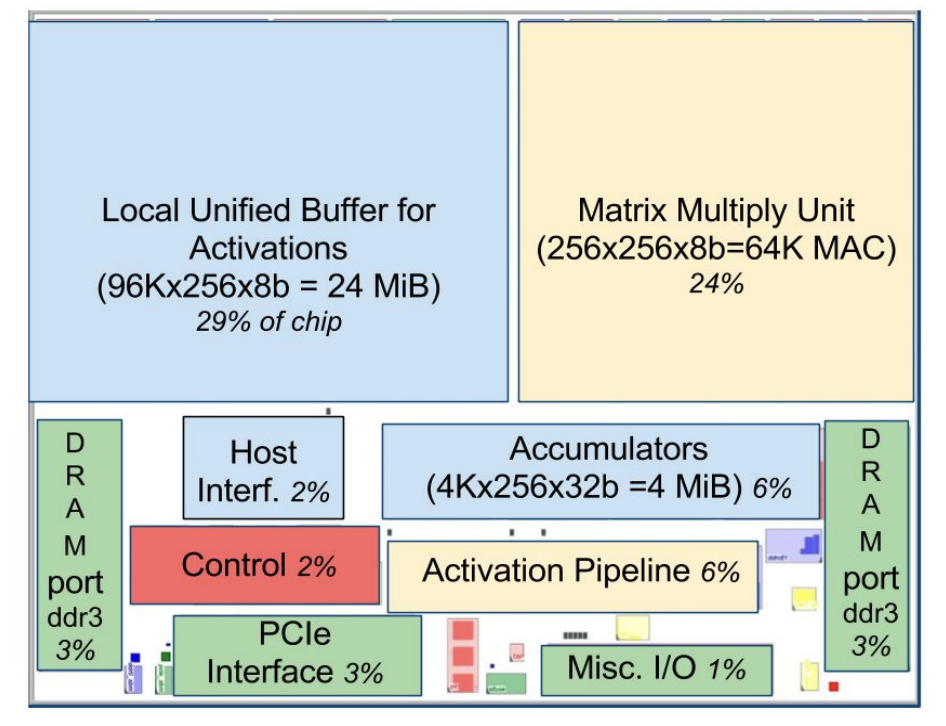
\includegraphics[scale=0.7]{floor-plan}
	\centering
	\caption{Divisão do uso do chip na TPU por unidade}
\end{figure}

Note que, a unidade de processamento de matrizes irá receber muitos dados de entrada, e ler dados da SRAM consome muito mais energia do que processamento aritmético, portanto essa unidade se aproveita de execução sistólica para economizar energia, reduzindo operações de leitura e escrita do Buffer unificado, dependendo de dados provindos de diversas direções alimentando um array em intervalos regulares.

\section{Principais instruções}

Como vimos, as instruções a serem executadas são enviadas de maneira externa para a TPU, através de PCIe (Peripheral Component Interconnect Express), o que pode ser relativamente lento e caminhar na direção oposta ao que é esperado. Nesse contexto, a fim de acelerar esse processo, a TPU utiliza da arquitetura CISC para definir instruções. A seguir, vemos algumas das principais instruções presentes na TPU:

$\bullet$ Read\_Host\_Memory: lê dados da CPU para o Buffer Unificado da TPU

$\bullet$ Read\_Weights: lê a entrada da unidade matricial

$\bullet$ MatrixMultiply/Convolve: faz com que a unidade matricial performe uma operação de multiplicação ou convolução, e deposite a saída nos acumuladores. Tal operação matricial leva tempo $B \times 256$ da entrada, multiplica por uma constante $256 \times 256$ e produz uma saída de tamanho $B \times 256$, e leva $B$ ciclos de clock para ser concluída.

$\bullet$ Activate: performa a função não linear de ativação no neurônio processado que está no acumulador, podendo ser, nativamente, ReLU, Sigmoid, até mesmo pooling para convoluções. Sua saída é levada para o Buffer unificado.

$\bullet$ Write\_Host\_Memory: escreve os dados do Buffer unificado na CPU.

Como podemos ver, essas principais instruções giram em torno do uso da unidade de processamento de matriz, além de trazer a aplicação de funções conhecidas de Machine Learning, como pooling e funções de ativação, para serem executadas a nível de hardware, acelerando ainda mais o processo. A filosofia geral da TPU é manter a unidade de matrizes sempre ocupada, e processar diversas instruções paralelamente, para evitar que a unidade de matrizes não tenha entrada assim que acabar uma operação.

\section{Compatibilidade}

Note que a TPU está sendo utilizada sempre de maneira conjunta com a CPU, para recebimento de dados a serem processados. Dessa forma, a pilha de software da TPU tinha como necessidade padrão ser compatível com softwares feitos para rodar na CPU e GPU. Para evitar problemas de compatibilidade, a aplicação de roda na TPU é feita utilizando TensorFlow e compilada em uma API que é capaz de rodar na CPU e GPU.

\begin{figure}[h]
	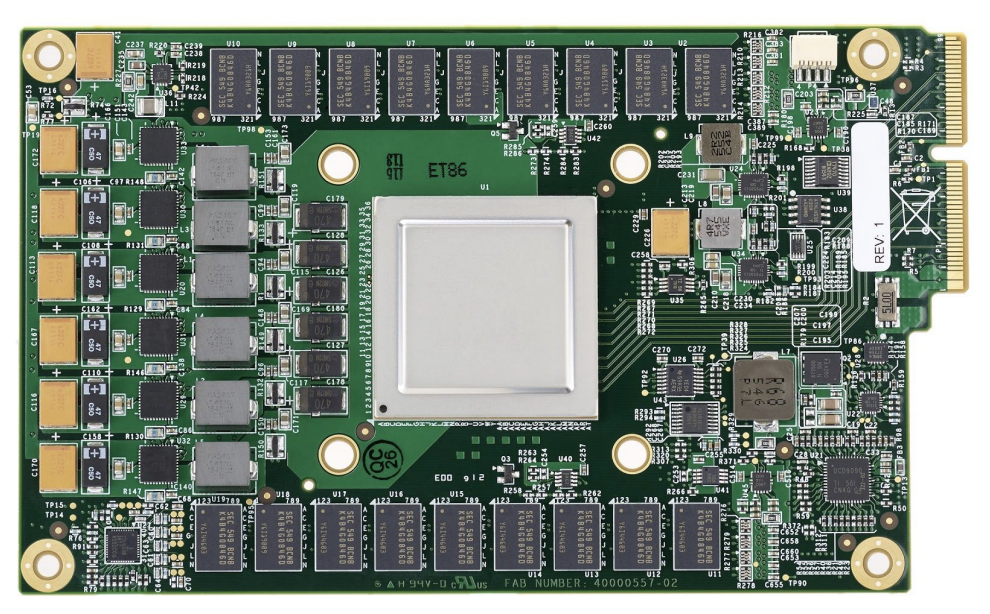
\includegraphics[scale=0.7]{circuit-board}
	\centering
	\caption{Placa de circuito da TPU}
\end{figure}

% --- CHAPTER 6 --- % 
\chapter{TPU vs GPU}

% --- CHAPTER 7 --- % 
\chapter{TensorFlow}

% --- CHAPTER 8 --- % 
\chapter{Cloud TPU v5p}

Como discutido anteriormente, LLMs são os novos modelos mais explorados no mercado e na academia. Todavia, esses modelos utilizam dados de toda (ou quase toda) a internet, que cresce ainda mais exponencialmente. Todos os dias há milhões de novos dados sendo gerados. Dessa forma, é importante que o hardware acompanhe o crescimento na quantidade de dados disponíveis, de forma que seja possível possuir poder computacional suficiente para treinar modelos como esses.

Com isso em vista, a evolução das TPUs deve ser rápida, portanto, em 2023, a Google apresentou, em 2023, a v5p, a TPU mais poderosa da empresa. Com esse lançamento, a Google prometeu a entrega de uma performance até $2.8$ vezes mais rápida, utilizada para alimentar ecossistemas internos da multinacional, como o Youtube, Android e Gmail.

Essa TPU se diferencia das demais, pois é focada em desempenho possível, sem levar em consideração a facilidade operacional. Um grande diferencial é a forma como a TPU lida com operações em ponto flutuante. Por dados oficiais da Google, essa arquitetura traz $8960$ chips e três vezes mais memória HBM.

\begin{figure}[h]
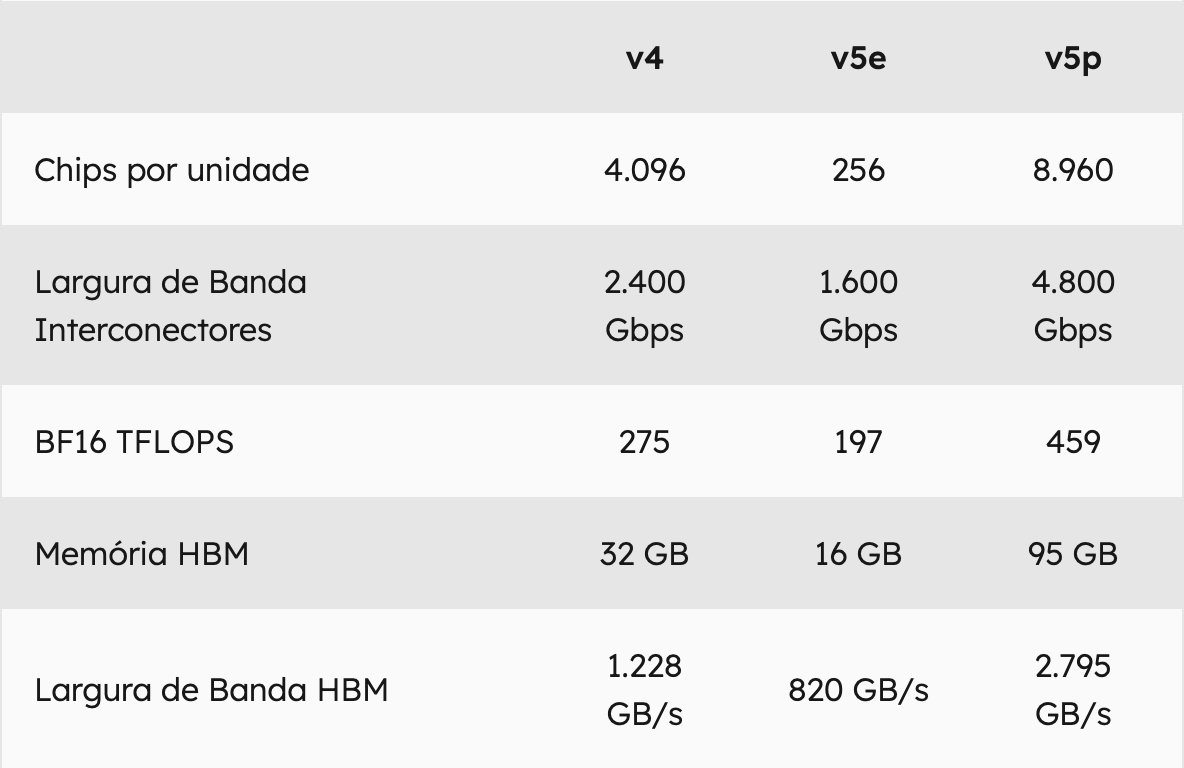
\includegraphics[scale=0.7]{comparativo-tpus}
\centering
\caption{Comparativo entre TPUs Google para cargas de trabalho em IA e LLM}
\end{figure}

Mas no fim, o que significam esses valores? A Google promete que a nova TPU consegue escalar o tempo de treinamento, sendo até $4X$ mais rápida que TPUs mais baratas, como a $V4$, devido ao dobramento no tamanho de operações em ponto flutuante que são entregues.

% --- CHAPTER 9 --- % 
\chapter{Consumo de Energia}

Atualmente, TPUs são encontradas com maior frequência em data centers, e são um produto extremamente utilizado não só pela Google, como também por empresas e usuários que dependem de seus serviços de nuvem.

Para avaliar, primeiramente, a performance/watt da TPU, e comparar com outras arquiteturas como GPU, se utiliza as métricas "total" (que calcula a energia consumida pela TPU/GPU juntamente a CPU, quando calcula performance/watt) e "incremental" (que subtrai a energia consumida pela CPU). A figura abaixo ilustra bem os resultados obtidos pela Google, que mostram uma performance de $17$ a $34$ vezes melhor que a GPU no modelo total, e de $25$ a $29$ vezes melhor que a GPU no modelo incremental.

\begin{figure}[h]
	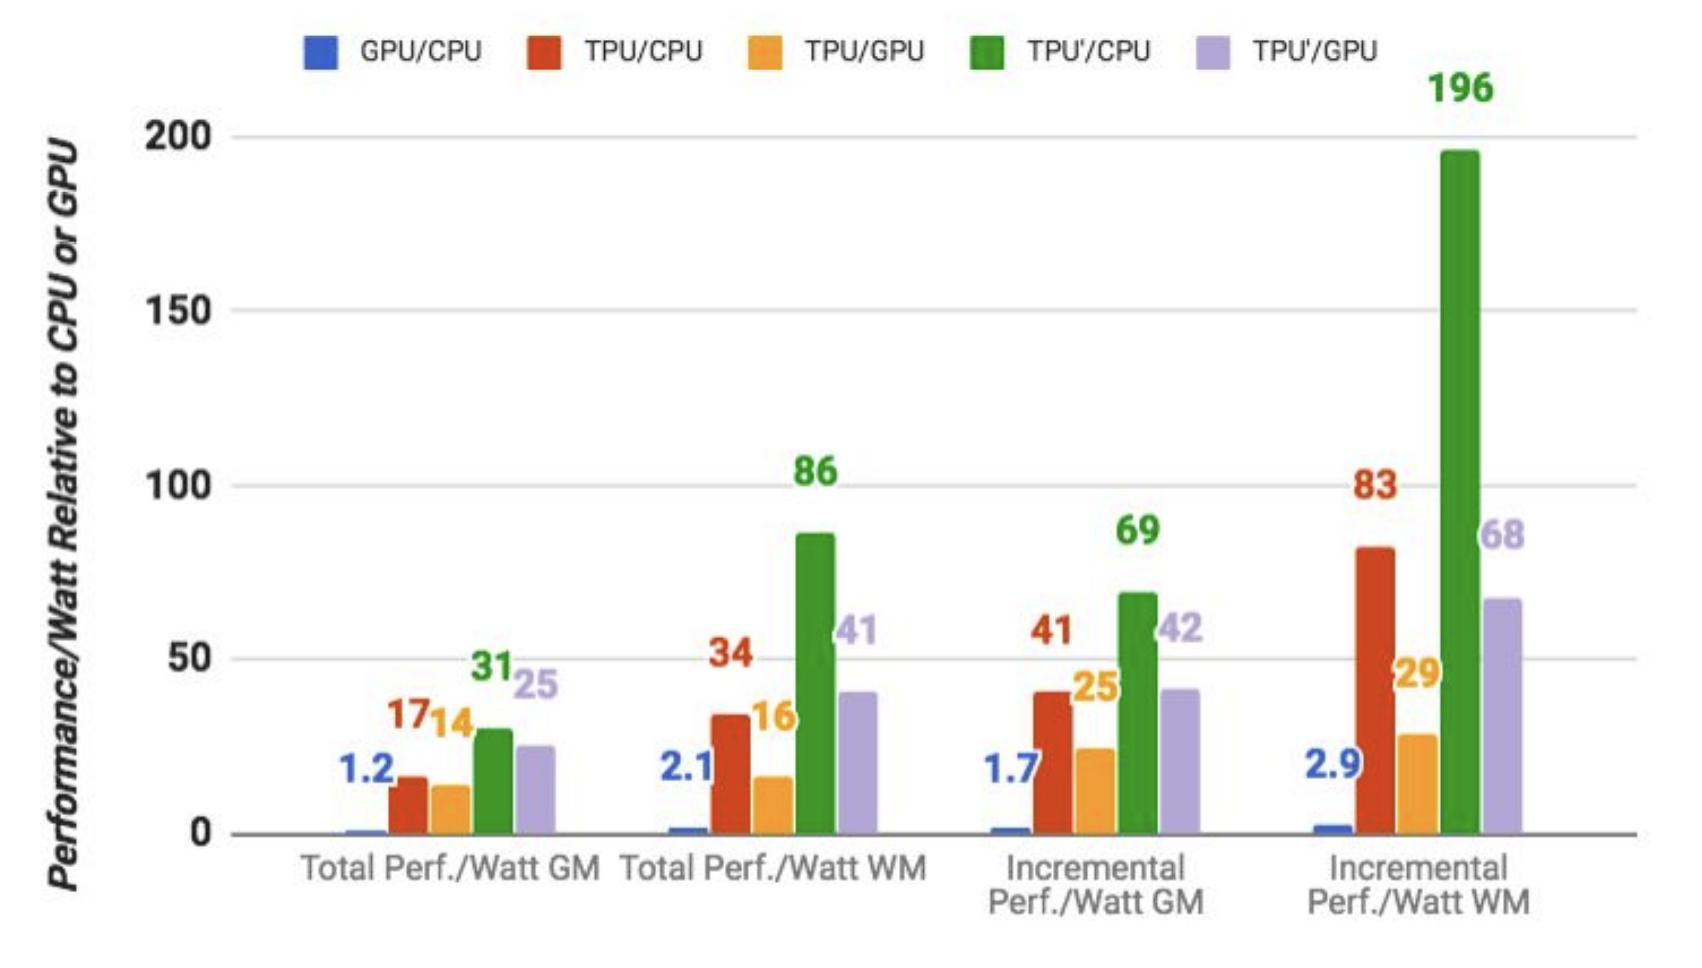
\includegraphics[scale=0.5]{performance-watt}
	\centering
	\caption{Performance/Watt para operações de médias geométricas e ponderadas (GM e WM, respectivamente)}
\end{figure}

Tendo esses consumos em vista, uma das medidas adequadas para se medir juntamente ao surgimento de uma nova arquitetura é o TDP (Thermal Design Power), que afeta diretamente o custo de energia gasto, tendo em vista que é necessário que a unidade receba energia e resfriamento suficientes. Tendo em vista que servidores não estão em funcionamento durante $100\%$ do tempo, é interessante que a energia consumida por essas máquinas seja proporcional ao seu tempo de uso.

A fim de medir tal consumo e avaliar a validade energética do uso de TPUs em detrimento de GPUs, a figura a seguir compara a energia gasta pelo servidor dividido pelo número de dias, variando o workload para processar CNN0, utilizando o mesmo batch para todos os testes.

\begin{figure}[h]
	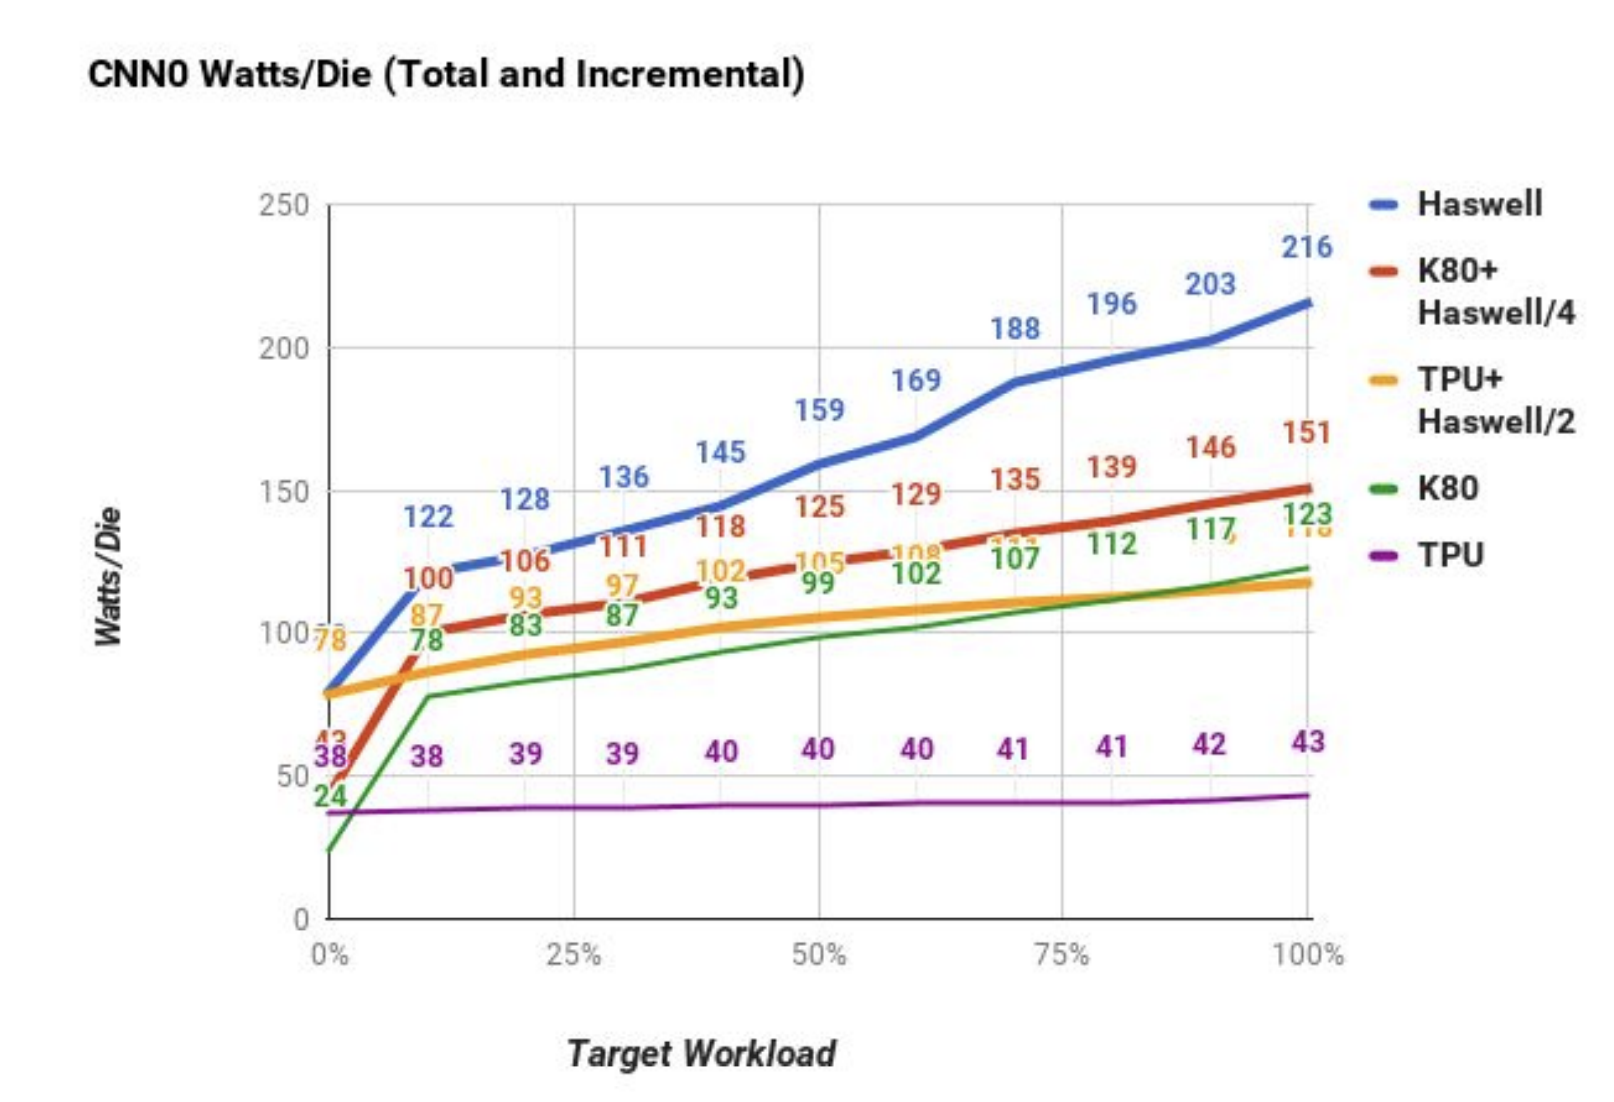
\includegraphics[scale=0.5]{watts-die}
	\centering
	\caption{Performance/Watt para operações de médias geométricas e ponderadas (GM e WM, respectivamente)}
\end{figure}


Pelos resultados obtidos, vemos que as TPUs conseguem consumir, no geral, menos energia que as GPUs, porém há um trade-off grande, pois a quantidade de energia consumida, mesmo com pouca operação na máquina, ainda é muito similar ao consumo com a máquina funcionando em $100\%$. Ou seja, quando a TPU e GPU estão totalmente carregadas, o servidor de CPU gasta $52\%$ da energia da GPU e $69\%$ da energia da TPU. Nesse sentido, a TPU ainda gasta mais energia proporcionalmente, pois realiza muito mais tarefas que a GPU, porém seus gastos em valor absoluto ainda são inferiores, e justificam o uso desse hardware.

% --- CHAPTER 10 --- % 
\chapter{Considerações Finais}

\bibliographystyle{alpha}
\bibliography{sample}

\href{https://www.run.ai/guides/cloud-deep-learning/google-tpu}{TPU e Arquitetura}

\href{https://cloud.google.com/blog/products/compute/performance-per-dollar-of-gpus-and-tpus-for-ai-inference}{Comparativos oficiais em modelos de IA (TPU vs GPU)}

\href{https://canaltech.com.br/inteligencia-artificial/cloud-tpu-v5p-e-o-novo-e-mais-poderoso-acelerador-de-ia-do-google-272299/}{TPU v5p}

\href{https://cloud.google.com/tpu?hl=pt-BR}{Conceitos básicos}

\href{https://en.wikipedia.org/wiki/Tensor_Processing_Unit}{Wikipedia, tem tudo}

\href{https://arxiv.org/pdf/1704.04760}{Paper original da TPU}

\end{document}